%%
%% (
%%  )\ )                             (
%%  (()/(   (            (             )\  )   (
%%   /(_))  ))\   (       ))\  (   (   (()/(   ))\
%%   (_))  /((_)  )\  )  /((_) )\  )\   ((_))/((_)
%%   | _ \(_))(  _(_/( (_) )  ((_)((_)  _| |(_))
%%   |   /| || || ' \))/ -_)/ _|/ _ \/ _` |/ -_)
%%   |_|_\ \_,_||_||_| \___|\__|\___/\__,_|\___|
%%

\documentclass{article}
\usepackage[utf8x]{inputenc}
\usepackage{amsmath}
%\usepackage{slashbox}
\usepackage{amsfonts}
\usepackage{amssymb}
\usepackage{graphicx} % Paquete para incluir imágenes en el documento LaTeX
\usepackage{hyperref}
\hypersetup{
  colorlinks=true,
  linkcolor=blue,
  filecolor=magenta,
  urlcolor=cyan,
}
\urlstyle{same}
\usepackage{varwidth}

\newcommand\tab[1][1cm]{\hspace*{#1}}

\usepackage{multirow}

\usepackage[a4paper,rmargin=1.5cm,lmargin=1.5cm,top=1.5cm,bottom=1.5cm]{geometry}

\usepackage{pdfpages}

\usepackage{xcolor}
\usepackage{minted}
\setminted[css]{frame=lines, framesep=2mm, baselinestretch=1.2, rulecolor=\color{black!80},
                bgcolor=DarkGray,fontsize=\normalsize}
\usemintedstyle[css]{monokai}
\setminted[python]{frame=lines, framesep=2mm, baselinestretch=1.2, rulecolor=\color{black!80}, bgcolor=DarkGray}
\usemintedstyle[python]{monokai}
\setminted[java]{frame=lines, framesep=2mm, baselinestretch=1.2, rulecolor=\color{black!80}, bgcolor=DarkGray}
\usemintedstyle[java]{monokai}
\setminted[javascript]{frame=lines, framesep=2mm, baselinestretch=1.2, rulecolor=\color{black!80}, bgcolor=DarkGray}
\usemintedstyle[javascript]{monokai}
\setminted[php]{frame=lines, framesep=2mm, baselinestretch=1.2, rulecolor=\color{black!30}, bgcolor=LightGray}
\setminted[html]{frame=lines, framesep=2mm, baselinestretch=1.2, rulecolor=\color{black!30}, bgcolor=LightGray}
\setminted[bash]{baselinestretch=1.2,rulecolor=\color{black!30},bgcolor=LightGray}
\definecolor{LightGray}{gray}{0.90}
\definecolor{DarkGray}{gray}{0.1}
\definecolor{MidGray}{gray}{0.8}
\definecolor{codegreen}{rgb}{0,0.6,0}
\definecolor{codegray}{rgb}{0.5,0.5,0.5}
\definecolor{codepurple}{rgb}{0.58,0,0.82}
\definecolor{backcolour}{rgb}{0.95,0.95,0.92}
\setminted[json]{frame=lines, framesep=2mm, baselinestretch=1.2, rulecolor=\color{black!80}, bgcolor=DarkGray}
\usemintedstyle[json]{monokai}
\setminted[apacheconf]{frame=lines, framesep=2mm, baselinestretch=1.2, rulecolor=\color{black!30}, bgcolor=LightGray}
\setminted[html+twig]{frame=lines, framesep=2mm, baselinestretch=1.2, rulecolor=\color{black!30}, bgcolor=LightGray}
\setminted[html+php]{frame=lines, framesep=2mm, baselinestretch=1.2, rulecolor=\color{black!30}, bgcolor=LightGray}

\setlength{\parindent}{0px}  % Setea la indentacion de la primera linea de cada parrafo a cero pixeles.


\title{Programación en Python 2}
\author{@RuneCode}

\begin{document}
%% Portada
\includepdf{./portada/portada.pdf}

%% Clase previa #1
\section*{Instalación de anaconda}%

Para descargar anaconda puedes visitar el siguiente
\href{https://www.anaconda.com/}{enlace}.

\begin{figure}[h!]
  \centering
  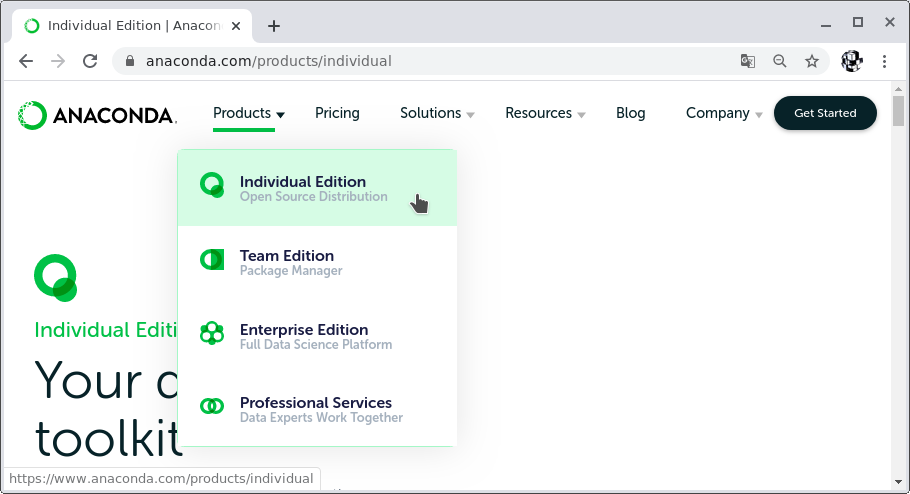
\includegraphics[scale=0.75]{./Pictures/001_install_anaconda.png}
\end{figure}

\begin{figure}[h!]
  \centering
  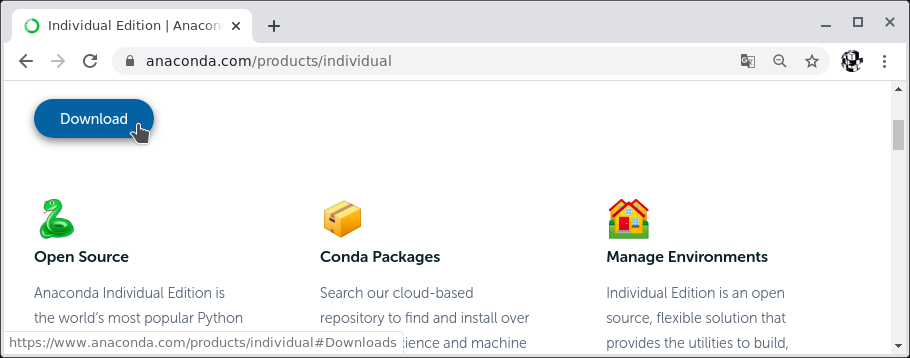
\includegraphics[scale=0.75]{./Pictures/001_download_anaconda.png}
\end{figure}

\newpage

\begin{figure}[h!]
  \centering
  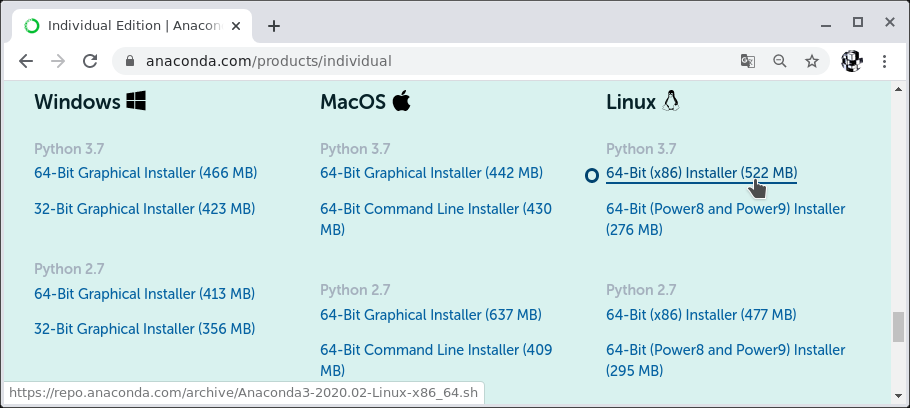
\includegraphics[scale=0.75]{./Pictures/002_download_anaconda.png}
\end{figure}

Al descargar obtendremos un script bash llamado
\textbf{Anaconda3-2020.02-Linux-x86\_64.sh}. Para poder ejecutarlo agregamos el
permiso de ejecución usando \textbf{chmod}\\

\begin{minted}{bash}
  chmod 755 Anaconda3-2020.02-Linux-x86_64.sh
  ./Anaconda3-2020.02-Linux-x86_64.sh
\end{minted}


\begin{figure}[h!]
  \centering
  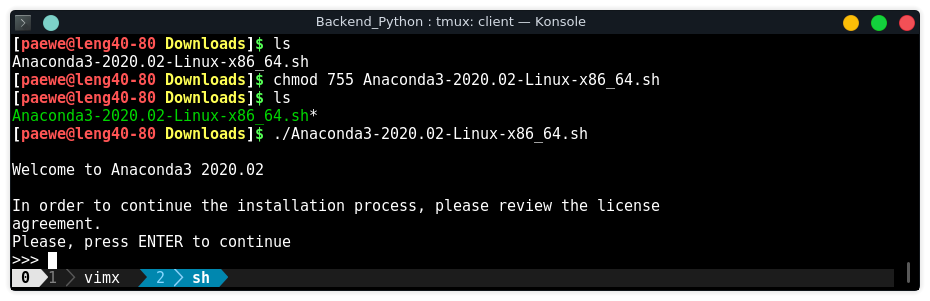
\includegraphics[scale=0.75]{./Pictures/003_install_anaconda.png}
\end{figure}

Para recorrer el acuerdo de licencia debes presionar la tecla \textbf{Espacio}
varias veces.

\begin{figure}[h!]
  \centering
  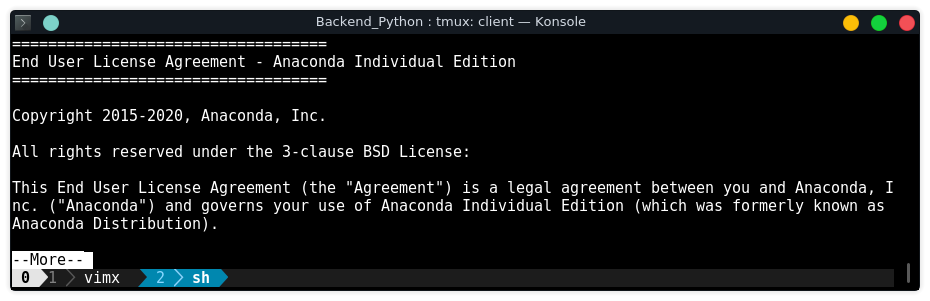
\includegraphics[scale=0.75]{./Pictures/004_licencia_more.png}
\end{figure}

\newpage

Para aceptar los terminos de la licencia escribimos \textbf{yes}.

\begin{figure}[h!]
  \centering
  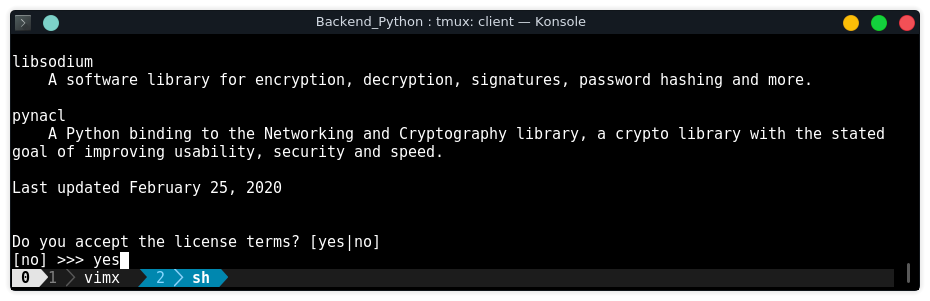
\includegraphics[scale=0.75]{./Pictures/005_aceptar_licencia.png}
\end{figure}

Luego escogemos un locación donde guardaremos anaconda o si queremos
simplemente presionamos \textbf{Enter} para usar la locación por defecto.

\begin{figure}[h!]
  \centering
  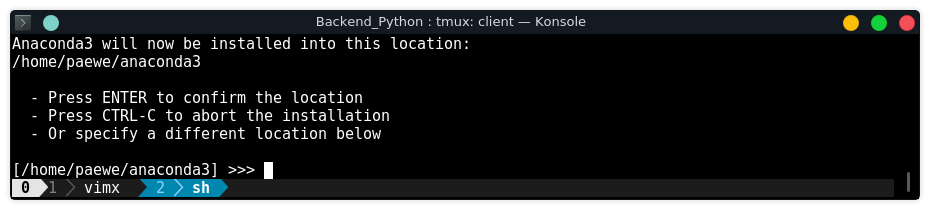
\includegraphics[scale=0.75]{./Pictures/006_install_location.png}
\end{figure}

Escogemos la opción \textbf{yes} para iniciar anaconda cada vez que se inicie
bash.

\begin{figure}[h!]
  \centering
  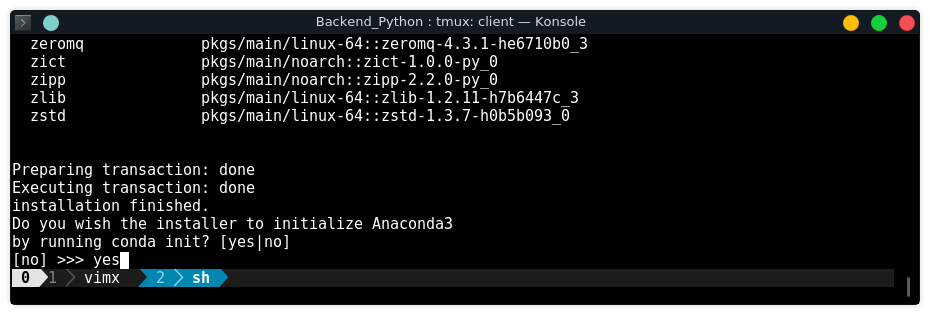
\includegraphics[scale=0.75]{./Pictures/007_iniciar_bash.png}
\end{figure}

Finalmente con esto ya se ha completado la instalación. Pero podemos configurar conda para que aunque se inicie no nos muestre el mensaje \textbf{base} en la parte izquierda del prompt. Para eso usamos:

\begin{minted}{bash}
  conda config --set changeps1 False
\end{minted}

Esto nos crea un archivo llamado \textbf{.condarc} que guarda las
configuraciones usados por conda.

\newpage

\begin{figure}[h!]
  \centering
  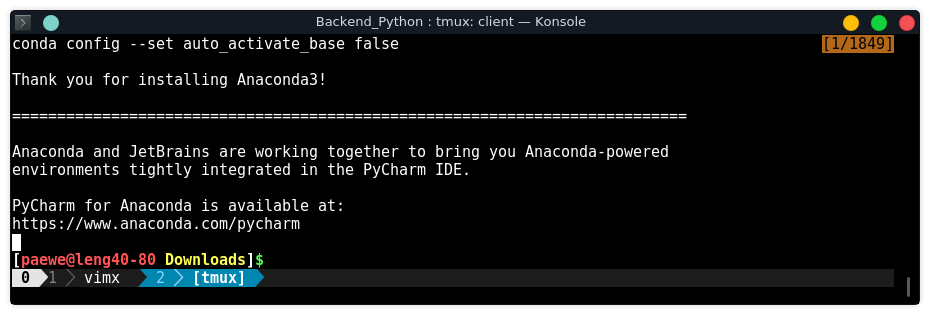
\includegraphics[scale=0.75]{./Pictures/008_instalacion_finalizada.png}
\end{figure}

\begin{figure}[h!]
  \centering
  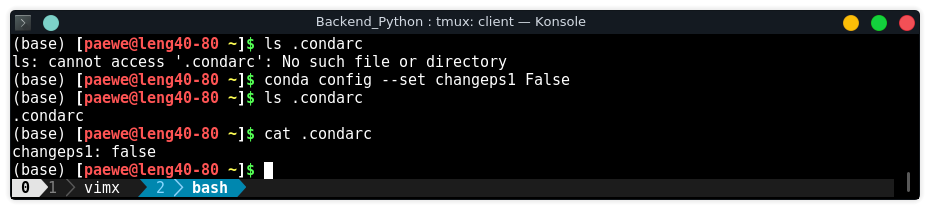
\includegraphics[scale=0.75]{./Pictures/009_changeps1_false.png}
\end{figure}

\newpage

%% Clase previa #2
\section*{Instalación de un nuevo entorno con python2}%

Ya que hemos descargado \textbf{Anaconda} con la versión de Python 3.7, si
queremos usar otra versión de Python podemos crear un nuevo entorno con la
versión que usaremos. Para mayor información puedes revisar la documentación de
\textbf{Conda} en el siguiente
\href{https://docs.conda.io/projects/conda/en/latest/user-guide/tasks/manage-environments.html#creating-an-environment-with-commands}{enlace}.\\

Escribimos el siguiente comando:

\begin{minted}{bash}
  conda create -n python2 python=2.7
\end{minted}

\begin{figure}[h!]
  \centering
  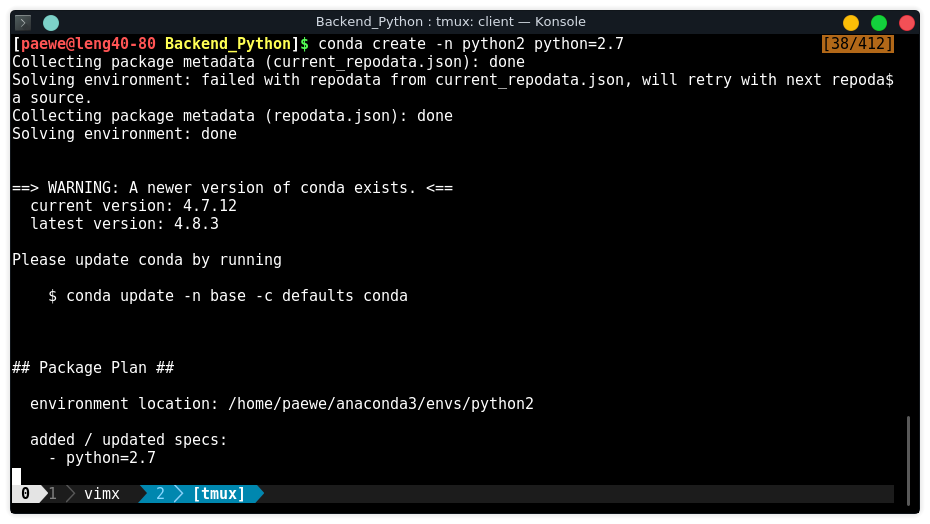
\includegraphics[scale=0.75]{./Pictures/001_crear_env_python2.png}
\end{figure}

\begin{figure}[h!]
  \centering
  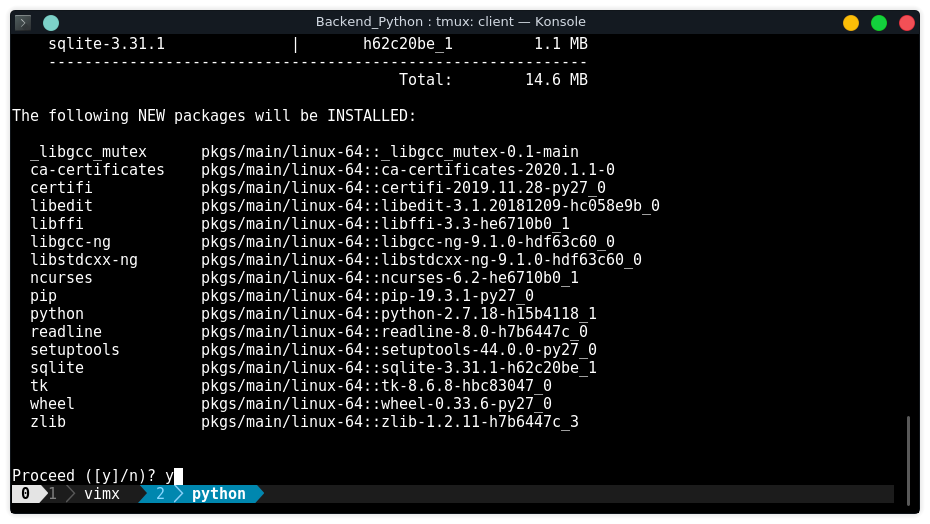
\includegraphics[scale=0.75]{./Pictures/002_crear_env_python2.png}
\end{figure}

\newpage

\begin{figure}[h!]
  \centering
  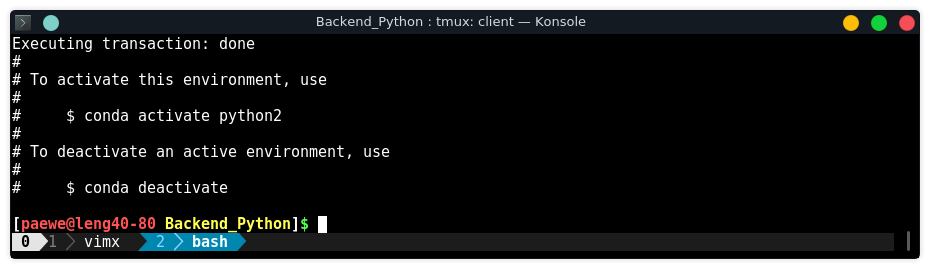
\includegraphics[scale=0.75]{./Pictures/003_crear_env_python2.png}
\end{figure}

Para activar el entorno que creamos usamos el siguiente comando.

\begin{minted}{bash}
  conda activate python2
\end{minted}

De igual manera, si queremos desactivar este entorno y usar el predeterminado
con Python 3.7, entonces usamos:

\begin{minted}{bash}
  conda deactivate
\end{minted}


\begin{figure}[h!]
  \centering
  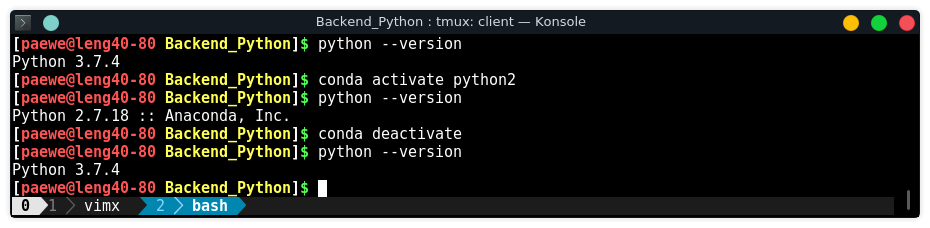
\includegraphics[scale=0.75]{./Pictures/004_activar_python2_desactivar.png}
\end{figure}

Si queremos ver los entornos que tenemos creados con Anaconda usamos el
siguiente comando:

\begin{minted}{bash}
  conda env list
\end{minted}


\begin{figure}[h!]
  \centering
  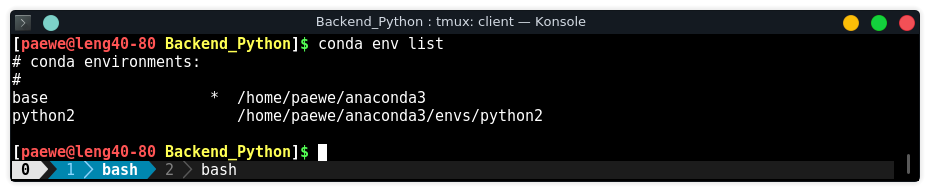
\includegraphics[scale=0.75]{./Pictures/005_ver_entornos_conda.png}
\end{figure}

\newpage

%% Clase 1
\section{¿Por qué programar con Python?}%
\subsection{¿Por qué?}%
Python es un lenguaje bastante bueno para aprender a programar ya que tiene una
comunidad muy grande que te ayudará a superar tus dudas, tiene una sintaxis
para escribir bastante sencilla.

\subsection{¿Qué es programar?}%
Programar es darle instrucciones al computador, para hacer algo que tu quieres,
desde tu sitio web a llevar humanos a marte.\\

Para lograr construir lo que quieres debes unir piezas básicas del lenguaje y
dependiendo de como las unas vas a construir eso que imaginas.\\

Para crear tu primer hola mundo debes encender el intérprete del Python, este
hola mundo es muy sencillo, ejecuta la función print así:

\begin{figure}[h!]
  \centering
  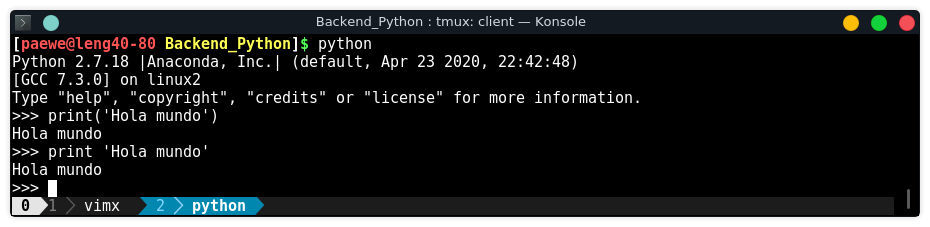
\includegraphics[scale=0.75]{./Pictures/005_hola_mundo_python2.png}
\end{figure}

Recuerda que la versión de Python que estaremos usando en el presente curso es
Python 2.


%% Clase 2
\section{¿Qué es la programación?}%
La programación es dar instrucciones a la computadora de forma ordenada, estas
instrucciones definen lo que se va a realizar, desde cosas sencillas hasta
cosas avanzadas.\\

Todos los programas se componen de partes esenciales que son forma de darle
datos de entrada a la computadora y formas estructuradas para procesar estos
datos.

\subsection{¿Cómo crearías un cuadrado?}%

Significa generar líneas y dar vueltas, ¿cómo escribes esto?. Hay una forma con
la librería \textbf{turtle}. Creamos el archivo:\\

\textbf{square.py}
\begin{minted}{python}
  import turtle

  window = turtle.Screen()
  david = turtle.Turtle()
  david.forward(150)
  david.left(90)
  david.forward(150)
  david.left(90)
  david.forward(150)
  david.left(90)
  david.forward(150)
  david.left(90)

  turtle.mainloop()
\end{minted}

Ejecutamos en la terminal bash:

\begin{minted}{bash}
  python square.py
\end{minted}


\begin{figure}[h!]
  \centering
  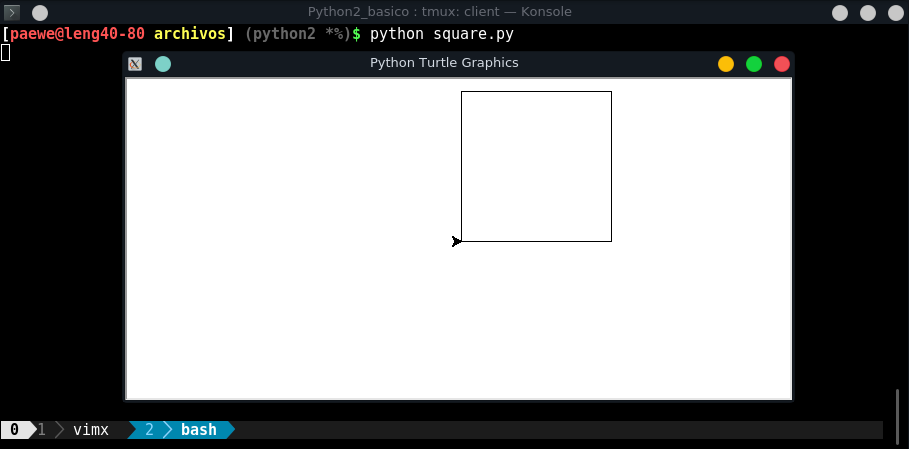
\includegraphics[scale=0.75]{./Pictures/011_square_turtle.png}
\end{figure}


%% Clase 3
\section{Guía de instalación y conceptos básicos}%
Puedes ver o descargar la guía visitando el siguiente
\href{https://drive.google.com/file/d/1Km1giTvN_waI59X0zvQ9akBxtsgqMrcR/view?usp=sharing}{enlace}.

%% Clase 4
\section{Operadores matemáticos en Python}%
Los operadores nos permiten trabajar con valores y generar nuevos valores por
medio de estas operaciones.\\

Existen muchos operadores básicos.
\begin{itemize}
  \item ($+$) Suma
  \item ($-$) Resta
  \item ($*$) Multiplicación
  \item ($/$) División
  \item ($//$) División de enteros
  \item ($\%$) Operador de módulo
  \item ($**$) Potencia
  \item ($>$) Mayor que
  \item ($<$) Menor que
  \item ($==$) Igual
  \item ($>=$) Mayor igual
  \item ($<=$) Menor igual
\end{itemize}

\newpage

\begin{figure}[h!]
  \centering
  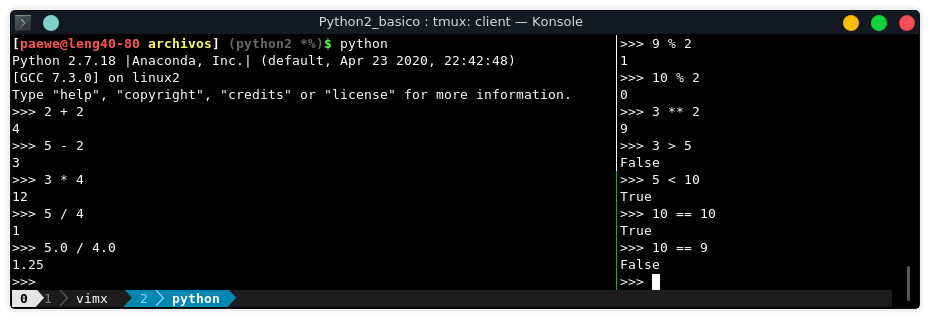
\includegraphics[scale=0.75]{./Pictures/012_operators.png}
\end{figure}

%% Clase 5
\section{Tipos de datos en Python}%
\subsection{¿En qué orden se evalúan las matemáticas operaciones complejas?}%

\begin{enumerate}
  \item Paréntesis xD
  \item Exponentes
  \item Multiplicación / División
  \item Adición / Sustracción
\end{enumerate}

Una forma fácil de recordar éste orden es usando el acrónimo PEMDAS:\\
(\textbf{P}aréntesis\textbf{E}xponentes\textbf{M}ultiplicación\textbf{D}ivisión\textbf{A}dición\textbf{S}ustracción)

\subsection{Valores y tipos}%
Los tipos le permiten a Python saber cuál es el resultado de aplicar
determinada operación, los tipos básicos son:

\begin{itemize}
  \item Integer $<$int$>$
  \item Float $<$float$>$
  \item String $<$str$>$
  \item Boolean $<$bool$>$
\end{itemize}

Para revisar de qué tipo es un dato puedes usar la función type.\\

Ejemplos:

\begin{figure}[h!]
  \centering
  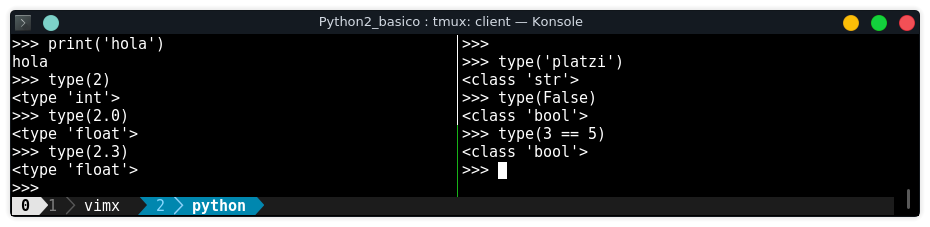
\includegraphics[scale=0.75]{./Pictures/013_tipos_datos.png}
\end{figure}

\newpage

%% Clase 6
\section{Declarar variables y expresiones}%
Las \textbf{variables} nos permiten guardar valores, permitiéndonos
reutilizarlos en diferentes partes del código y haciendo nuestros programas más
legibles.\\

El valor que contiene una variable puede ser reasignado, significa que podemos
asignarle diferentes valores a una misma variable.\\

Las variables tienen algunas limitantes, por ejemplo:

\begin{itemize}
  \item Tienen que tener un nombre significativo, es decir, que nos digan qué
    están haciendo.
  \item No podemos usar palabras reservadas del lenguaje como nombres para
    nuestras variables (por ejemplo class, false, none, true)
\end{itemize}

Para ver los \textbf{keywords} podemos usar \textbf{help()} que además nos
podría ayudar con los módulos, operadores y topicos.

\begin{minted}{bash}
  >>> help()
\end{minted}

\begin{figure}[h!]
  \centering
  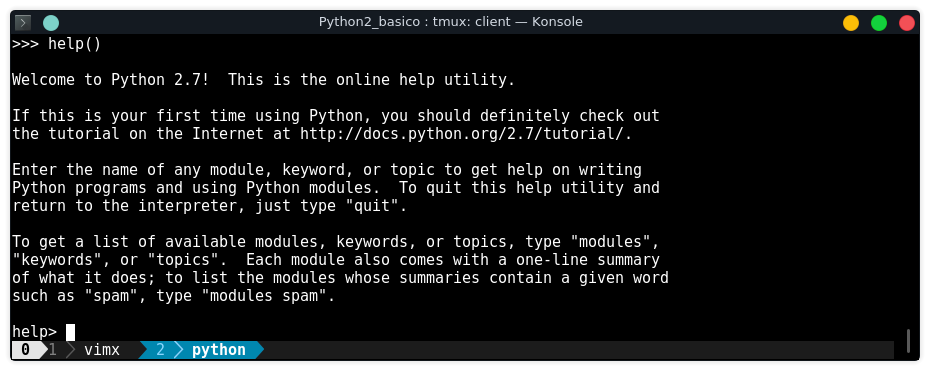
\includegraphics[scale=0.75]{./Pictures/014_help_python.png}
\end{figure}

Como indica en las instrucciones de la utilidad, escribimos \textbf{keywords} y
esto nos mostrará la lista de palabras clave.

\begin{minted}{bash}
  >>> keywords
\end{minted}

\begin{figure}[h!]
  \centering
  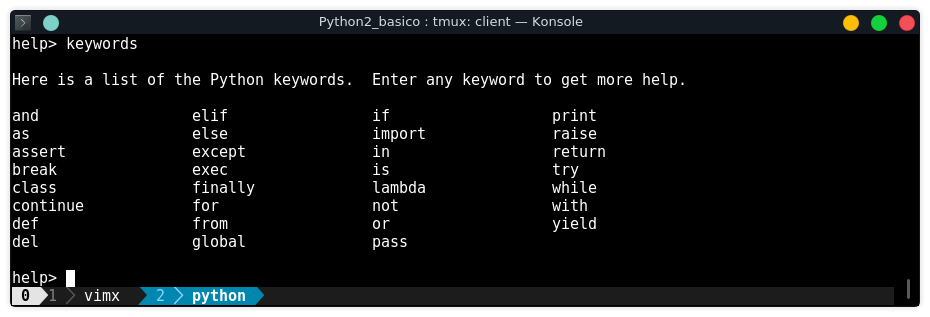
\includegraphics[scale=0.75]{./Pictures/015_keywords.png}
\end{figure}

\newpage

Para definir una variable escribes el nombre que quieres asignarle y con
\textbf{=} defines el valor que va a almacenar, por ejemplo:

\begin{figure}[h!]
  \centering
  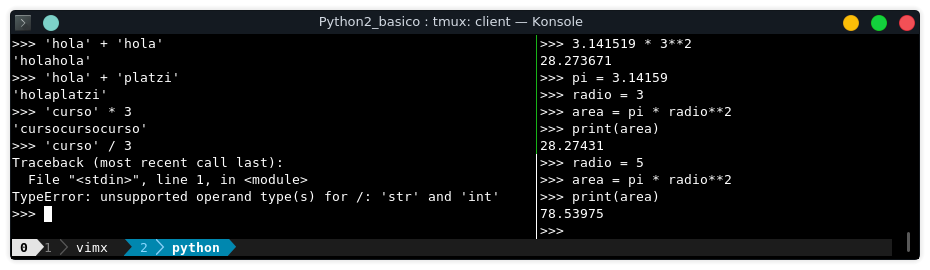
\includegraphics[scale=0.75]{./Pictures/016_tipo_de_datos_python.png}
\end{figure}

\subsection{Recuerda:}%
\begin{itemize}
  \item Todos los programas de Python deben guardarse con extensión
    \textbf{.py}
  \item Para darle soporte a acentos en nuestros programas debemos usar la
    \textbf{línea \# -*- coding: utf-8 -*-}
\end{itemize}

\textbf{saludos.py}
\begin{minted}{python}
  name = str(raw_input('¿Cuál es tu nombre? '))
  print('Hola, ' + name + '!')
\end{minted}

Para ejecutar el programa creado usamos:

\begin{minted}{bash}
  python saludos.py
\end{minted}

\begin{figure}[h!]
  \centering
  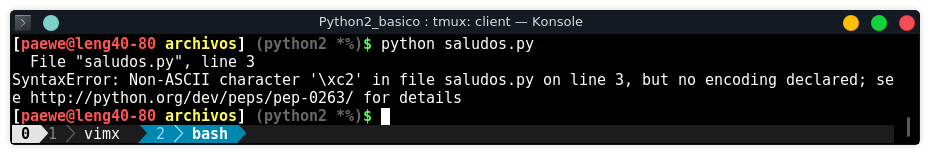
\includegraphics[scale=0.75]{./Pictures/017_saludos_ascii.png}
\end{figure}

Se observa un error relacionado al uso de caracteres no ASCII, Python 2 usa por
defecto caracteres ASCII, esto cambia en Python 3 ya que usa Unicode por
defecto. Para solucionar este error se agrega la línea \textbf{\# -*- coding:
utf-8 -*-} al principio.\\

\textbf{saludos.py}
\begin{minted}{python}
  # -*- coding: utf-8 -*-

  name = str(raw_input('¿Cuál es tu nombre? '))
  print('Hola, ' + name + '!')
\end{minted}

Ejecutamos nuevamente:

\begin{figure}[h!]
  \centering
  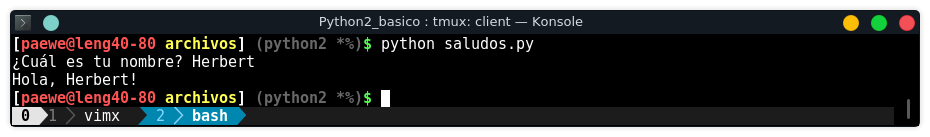
\includegraphics[scale=0.75]{./Pictures/018_saludos_exito.png}
\end{figure}

\newpage

%% Clase 7
\section{Definir funciones con Python}%
Las funciones son un concepto fundamental en programación, una función es una
secuencia de comandos que realizan un computo.\\

En Python las funciones se definen usando la palabra reservada \textbf{def} y
luego el nombre de la función con paréntesis y dos puntos que indican que lo
que sigue son los comandos, una función debe retornar un valor, para esto se
usa la palabra reservada \textbf{return}.

\begin{minted}{python}
  def suman(num1, num2):
    return num1 + num2
\end{minted}

Para usar una función simplemente la llamamos por su nombre seguido por
paréntesis con los parámetros que recibe.

\begin{minted}{python}
  suma(2, 3)
\end{minted}

Recuerda:
\begin{itemize}
  \item Si usas \textbf{Python 3}, debes usar la función \textbf{input()} para
    recibir datos del usuario.
  \item Para definir dónde comenzar el código usamos la línea. \textbf{if
    \_\_name\_\_ == '\_\_main\_\_'}
  \item Para definir un bloque dentro de la función debemos indentar con 4
    espacios.
  \item Las funciones nos permiten ejecutar determinado código con diferentes
    valores.
\end{itemize}


Vamos a refactorizar el programa para construir un cuadrado.\\

\textbf{functions.py}
\begin{minted}{python}
  # -*- coding: utf-8 -*-

  import turtle

  def main():
      window = turtle.Screen()
      dave = turtle.Turtle()

      make_square(dave)

      turtle.mainloop()


  def make_square(dave):
      lenght = int(raw_input('Tamaño de cuadrado: '))

      for i in range(4):
          make_line_and_turn(dave, lenght)


  def make_line_and_turn(dave, length):
      dave.forward(length)
      dave.left(90)


  if __name__ == '__main__':
      main()
\end{minted}

Ejecutamos el programa:

\begin{minted}{bash}
  python functions.py
\end{minted}

\begin{figure}[h!]
  \centering
  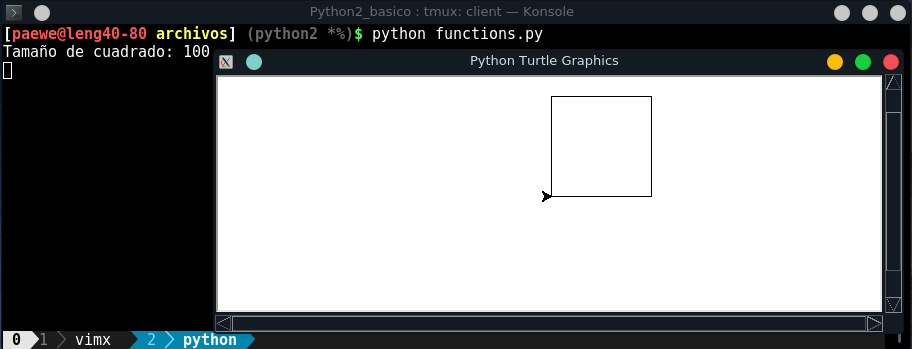
\includegraphics[scale=0.75]{./Pictures/023_function_square.png}
\end{figure}

\newpage

%% Clase 8
\section{Funciones con parámetros}%
\subsection{Límites al declarar funciones}%
\begin{itemize}
  \item Los nombres no pueden comenzar con dígitos.
  \item No pueden utilizar una palabra reservada.
  \item Las variables deben tener diferentes nombres.
  \item Los nombres de las funciones deben ser descriptivas de lo que hacen las
    funciones.
\end{itemize}

\subsection{Imprimir valor de variable}%
Para poder imprimir el valor de una variable dentro de un string podemos hacer
uso de \textbf{format}.

\subsection{Declarar vs Ejecutar}%
Declarar una función es escribir su estructura mientras que ejecutarla es
llamar a la función y ejecutar su código.

\subsection{Donde se puede acceder a las variables}%
Escope de las variables, cada vez que una función se ejecuta se genera un
contenedor donde las variables de la función van a vivir, una vez se sale de la
función estas variables no van a existir.\\

Por ejemplo vamos a trabajar en una calculadora de divisas:\\

\textbf{tipo\_cambio.py}
\begin{minted}{python}
  # -*- coding: utf-8 -*-

  def run():
      print('C A L C U L A D O R A  D E  D I V I S A S')
      print('Convierte pesos mexicanos a pesos colombianos.')
      print('')

      ammount = float(raw_input('Ingresa la cantidad de pesos mexicanos que quieres convertir: '))

      result = foreign_exchange_calculator(ammount)

      print('${} pesos mexicanos son ${} pesos colombianos'.format(ammount, result))


  def foreign_exchange_calculator(ammount):
      mex_to_col_rate = 145.97

      return mex_to_col_rate * ammount


  if __name__ == '__main__':
      run()
\end{minted}

Ejecutamos el programa:

\begin{minted}{bash}
  python tipo_cambio.py
\end{minted}

\newpage

\begin{figure}[h!]
  \centering
  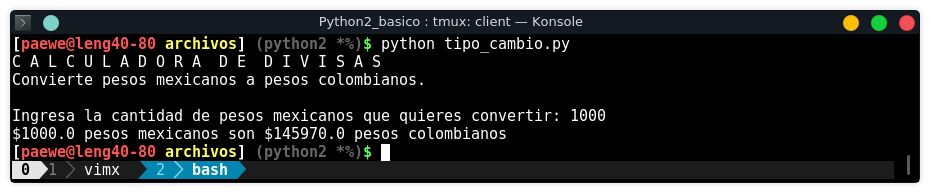
\includegraphics[scale=0.75]{./Pictures/024_funcion_tipo_cambio.png}
\end{figure}


%% Clase 9
\section{Estructura de condicionales en Python}%
Uno de las cosas más poderosas en programación es controlar el flujo de
ejecución, para esto utilizamos condicionales.\\

Las condicionales son sentencias que devuelven un valor booleano (True, False)\\

Podemos utilizar:

\subsection{Operadores relacionales}%
\begin{itemize}
  \item $==$ Es igual
  \item $!=$ Es diferente
  \item $>$ Es mayor
  \item $>=$ Es mayor o igual
  \item $<$ Es menor
  \item $<=$ Es menor o igual
\end{itemize}

\subsection{Operadores lógicos}%
\begin{itemize}
  \item and
  \item or
  \item not
\end{itemize}

Veamos en la shell de python:

\begin{figure}[h!]
  \centering
  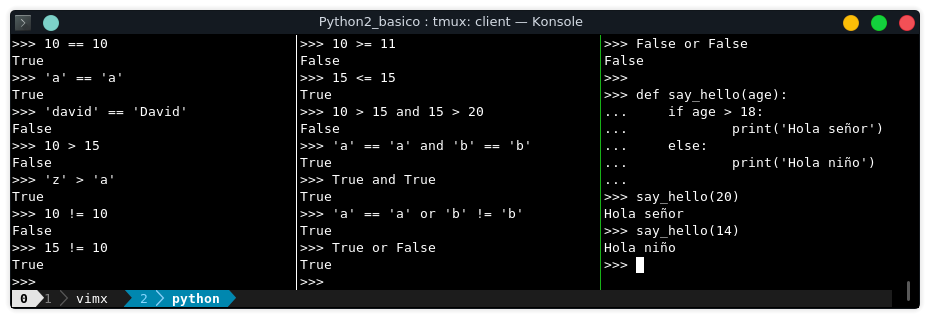
\includegraphics[scale=0.75]{./Pictures/025_relaciones_y_condicionales.png}
\end{figure}

\newpage


%% Clase 10
\section{Calcular si un número es primo con Python}%
En ésta clase vamos a construir un programa que nos permite determinar si un
número es primo o no, usando expresiones booleanas, operadores relacionales y
operadores lógicos.\\

\subsection{Recuerda:}%
\begin{itemize}
  \item Todas las funciones deben declararse con el keyword \textbf{def}.
  \item Un bug es un error en el código y requiere ser verificado.
\end{itemize}

\textbf{primo.py}
\begin{minted}{python}
  # -*- coding: utf-8 -*-


  def is_prime(number):
      if number < 2:
          return False
      elif number == 2:
          return True
      elif number % 2 == 0:
          return False
      else:
          for i in range(3, number):
              if number % i == 0:
                  return False
      return True


  def run():
      number = int(raw_input('Escribe un número: '))

      result = is_prime(number)

      if result is True:
          print('Tu número es primo')
      else:
          print('Tu número no es primo')


  if __name__ == '__main__':
      run()
\end{minted}

Ahora ejecutamos el programa:

\begin{minted}{bash}
  python primo.py
\end{minted}

\newpage

\begin{figure}[h!]
  \centering
  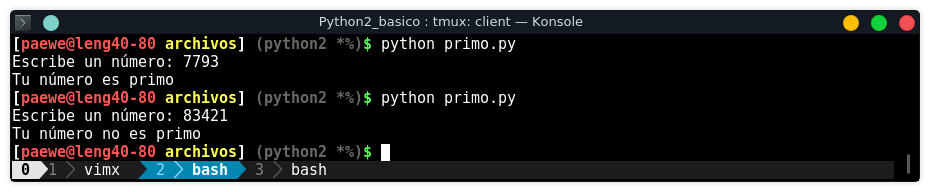
\includegraphics[scale=0.75]{./Pictures/026_primo.png}
\end{figure}

Hay varias formas de realizar el mismo algoritmo, así tenemos otra forma de
obtener si un número es primo o no usando Python.\\

\textbf{primo2.py}
\begin{minted}{python}
  # -*- coding: utf-8 -*-


  def is_prime(number):
      if number < 2:
          return False
      for x in range(2, number):
          if number % x == 0:
              return False
      else:
          return True


  def run():

      number = int(raw_input('Ingresa un número: '))

      result = is_prime(number)
      if result is True:
          print('{} es primo.'.format(number))
      else:
          print('{} no es primo.'.format(number))


  if __name__ == '__main__':
      run()
\end{minted}

Ahora ejecutamos el programa:

\begin{minted}{bash}
  python primo2.py
\end{minted}

\begin{figure}[h!]
  \centering
  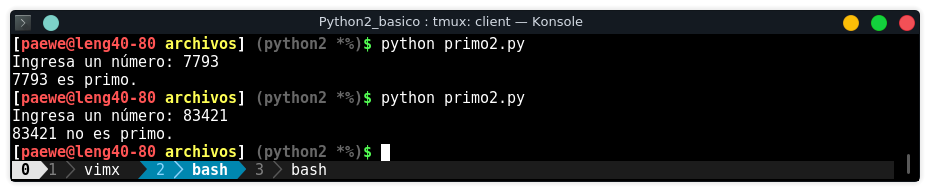
\includegraphics[scale=0.75]{./Pictures/027_primo2.png}
\end{figure}

\newpage

%% Clase 11
\section{Buena prácticas de lenguaje}%
Una forma de usar las condicionales es anidándolas. En este ejemplo vemos como
se pueden usar:
\textbf{genero.py}
\begin{minted}{python}
  # -*- coding: utf-8 -*-

  genero = raw_input("Ingresa tu genero: ")
  edad = int(raw_input("Ingresa tu edad: "))

  if genero == 'masculino':
      if edad > 18:
          print 'Hola, señor.'
      else:
          print 'Hola niño.'
  else:
      if edad > 18:
          print 'Hola, señora.'
      else:
          print 'Hola niña.'
\end{minted}

No es recomendable usar excesivamente este recurso. Hay que tener mucho cuidado
en no perder legibilidad de nuestro programa. Incluso en una de las frases zen
de Python nos indica que \textbf{Sencillo es mejor que anidado}.\\

Podemos ver el zen de Python en la misma shell:

\begin{figure}[h!]
  \centering
  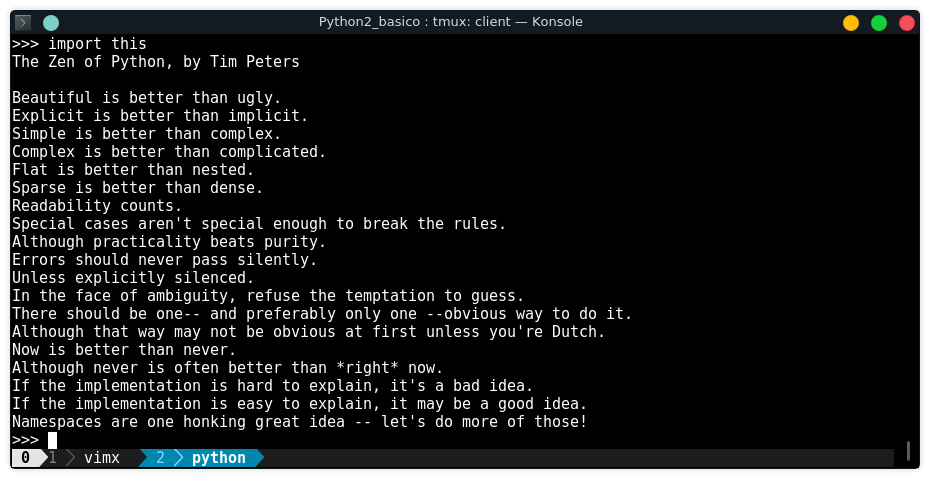
\includegraphics[scale=0.75]{./Pictures/028_import_this.png}
\end{figure}

Si traducimos el Zen de Python tenemos:

\begin{minted}{bash}
  Hermoso es mejor que feo.
  Explícito es mejor que implícito.
  Simple es mejor que complejo.
  Complejo es mejor que complicado.
  Sencillo es mejor que anidado.
  Escaso es mejor que denso.
  La legibilidad cuenta
  Los casos especiales no son lo suficientemente especiales como para romper las reglas.
  Sin embargo lo practico le gana a la pureza.
  Los errores no deben pasar en silencio.
  A menos que sean silenciados.
  Frente a la ambigüedad, evitar la tentación de adivinar.
  Debe haber una, y preferiblemente solo una, manera obvia de hacerlo.
  Aunque esa manera puede no ser obvia en un primer momento a menos que seas Holandés.
  Ahora es mejor que nunca.
  Aunque nunca es a menudo mejor que ahora mismo.
  Si la aplicación es difícil de explicar, es una mala idea.
  Si la aplicación es fácil de explicar, puede ser una buena idea.
  Los espacios de nombres son una gran idea, ¡hay que hacer más de eso!
\end{minted}

Si quieres profundizar mucho más en el lenguaje es recomendable leas su
documentación. Puedes encontrar su contenido visitando el siguiente
\href{https://docs.python.org/3/}{enlace}.


%% Clase 12
\section{Comparación de strings y unicode}%
Los strings tienen una característica muy importante: son inmutables, esto
quiere decir que no se pueden cambiar después de que se han declarado.\\

Si quieres modificar el texto de un string debes definir un nuevo string y
modificarlo usando funciones como slice.

\begin{figure}[h!]
  \centering
  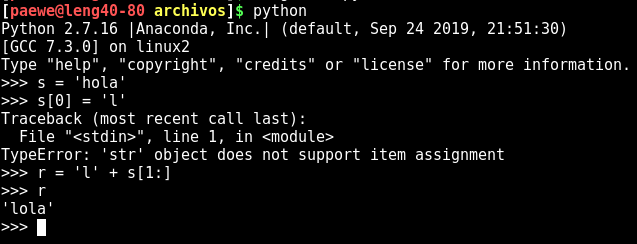
\includegraphics[scale=0.75]{./Pictures/001_string_inmutable.png}
\end{figure}

\textbf{Comparación de strings}: Se puede realizar operaciones con strings, por
ejemplo comparar si son iguales o mayores o menores.

\begin{figure}[h!]
  \centering
  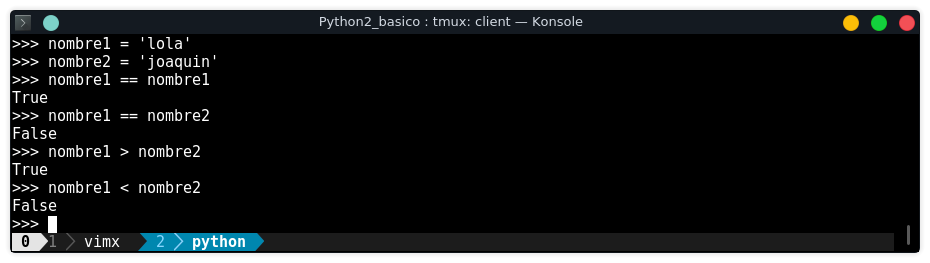
\includegraphics[scale=0.75]{./Pictures/002_comparar_strings.png}
\end{figure}

\textbf{Diferencia entre ASCII y Unicode}: Los caracteres también son números,
para esto existen estándares que asignan un número a cada carácter, para
generar un estándar se creó el ASCII pero esta solo toma en cuenta los
caracteres en inglés, para dar soporte a más lenguajes sea UNICODE.\\

Python 2 codifica en ASCII por default, para cambiarlo por UNICODE debemos
colocar u antes del string. Python 3 codifica en Unicode por defecto.

\newpage

\begin{figure}[h!]
  \centering
  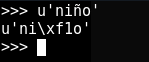
\includegraphics[scale=0.75]{./Pictures/003_unicode_python2.png}
\end{figure}


%% Clase 13
\section{Factorial de un número con recursión}%
Una función está siendo recursiva cuando dentro del bloque de instrucciones que
la conforma se usa a sí misma. El conceptop puede sonar complicado pero es muy
común su uso, por ejemplo cuando haces el cálculo del factorial de un número lo
haces con una función recursiva:\\

El factorial de un número es el número multiplicado por los números antes de
él, por ejemplo: $5! = 5*4*3*2*1$\\

Esto se puede expresar como:

\begin{minted}{python}
  5 * fac(4)
  4 * fac(3)
  3 * fac(2)
  2 * fac(1)
  1 * fac(0)
\end{minted}

Nota importante: Cuando estés trabajando con recursividad siempre debes pensar
en el caso base, es decir debes definir el momento en el que la función dejará
de llamarse a sí misma, para que no hagas un loop infinito, por ejemplo en el
caso del factorial terminas la ejecución cuando llegas a cero.\\

\textbf{factorial.py}
\begin{minted}{python}
  # -*- coding: utf-8 -*-

  def factorial(number):
      if number == 0:
          return 1

      return number * factorial(number - 1)


  if __name__ == '__main__':
      number = int(raw_input('Ingrese el número: '))
      result = factorial(number)

      print(result)
\end{minted}

\begin{figure}[h!]
  \centering
  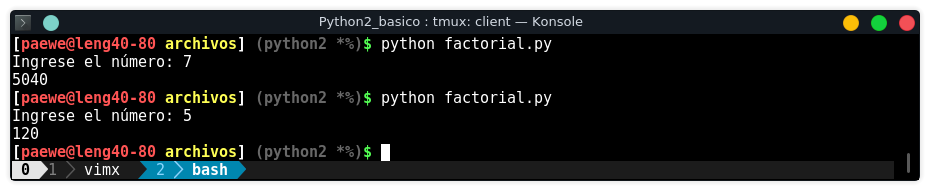
\includegraphics[scale=0.75]{./Pictures/029_factorial.png}
\end{figure}

\newpage


%% Clase 14
\section{Manejo de strings en Python}%
Un string es una secuencia de caracteres, donde cada caracter tiene un indice
que inicia en cero por ejemplo:

\begin{minted}{python}
  my_string = 'platzi'

  my_string[0] # p
  my_string[1] # l
  my_string[2] # a
  my_string[3] # t
  my_string[4] # z
  my_string[5] # i
\end{minted}

Para conocer la longitud de un string podemos usar la función \textbf{len}

\begin{minted}{python}
  len(my_string) # 6
\end{minted}

Los string tienen algunos métodos útiles como:

\begin{minted}{python}
  my_string.upper() # retorna el string en mayúsculas
  my_string.lower() # retorna el string en minúsucula
  my_string.find('F') # retorna el índice donde se encuentra
\end{minted}

\begin{figure}[h!]
  \centering
  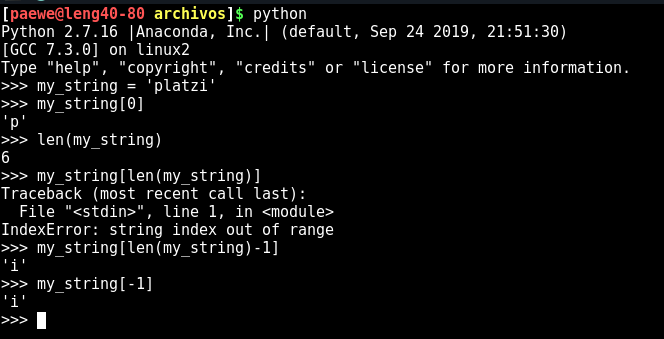
\includegraphics[scale=0.75]{./Pictures/004_index_string_len.png}
\end{figure}

Los métodos más conocidos:

\begin{itemize}
  \item upper
  \item iupper
  \item lower
  \item islower
  \item find
  \item isdigit
  \item endswith
  \item startswith
  \item split
  \item join
\end{itemize}

\begin{figure}[h!]
  \centering
  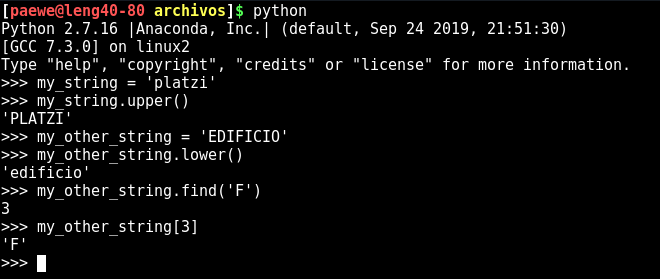
\includegraphics[scale=0.75]{./Pictures/005_methods_string.png}
\end{figure}


%% Clase 15
\section{Separar cadenas de texto en Python}%
La funcion \textbf{slice} de python nos permite separar los strings en
substrings generando nuevas secuencias.

\begin{minted}{python}
  my_string[inicio:fin:saltos]
\end{minted}

\begin{figure}[h!]
  \centering
  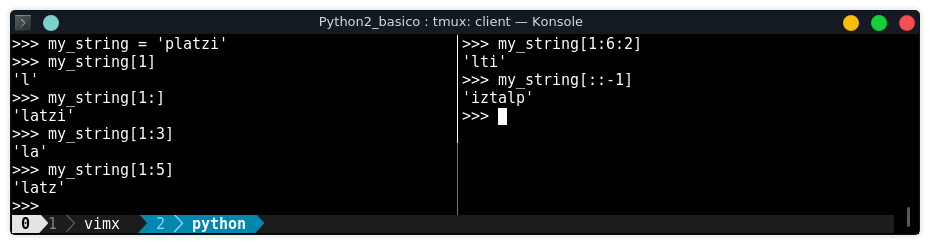
\includegraphics[scale=0.75]{./Pictures/019_slices.png}
\end{figure}


\newpage

%% Clase 16
\section{Ciclos en Python con for}%
Cuando necesitamos realizar operaciones sobre una serie de datos podemos
utilizar iteraciones.\\

\textbf{Función range}: La función range nos permite generar un string apartir
de un rango.\\

\textbf{Iteraciones con for}: for nos permite recorrer un arreglo,
asignando cada valor a una variable que decidas.

\begin{figure}[h!]
  \centering
  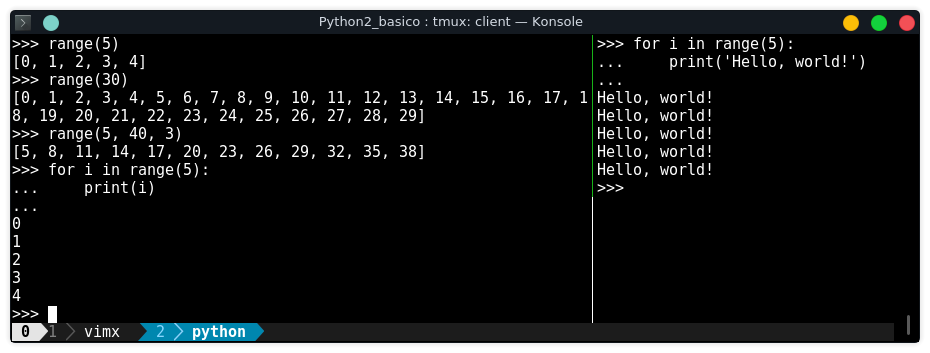
\includegraphics[scale=0.75]{./Pictures/020_range_for.png}
\end{figure}


Podemos operar los valores usando también condiciones, en este caso solo
queremos elevar al cuadrado, los valores que sean divisibles por 3.\\

La palabra reservada \textbf{continue} permite saltar a la siguiente iteración
del ciclo y \textbf{break} permite salirse del ciclo.

\begin{figure}[h!]
  \centering
  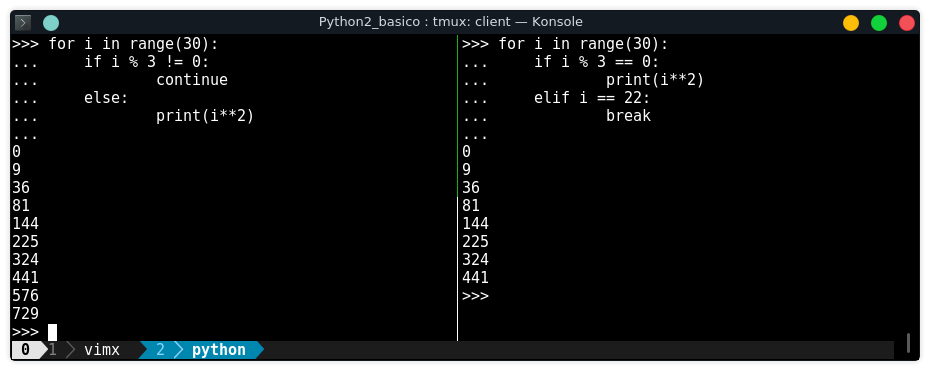
\includegraphics[scale=0.75]{./Pictures/021_for.png}
\end{figure}

También podemos recorrer los caracteres de una cadena de caracteres usando
\textbf{for}.

\newpage

\begin{figure}[h!]
  \centering
  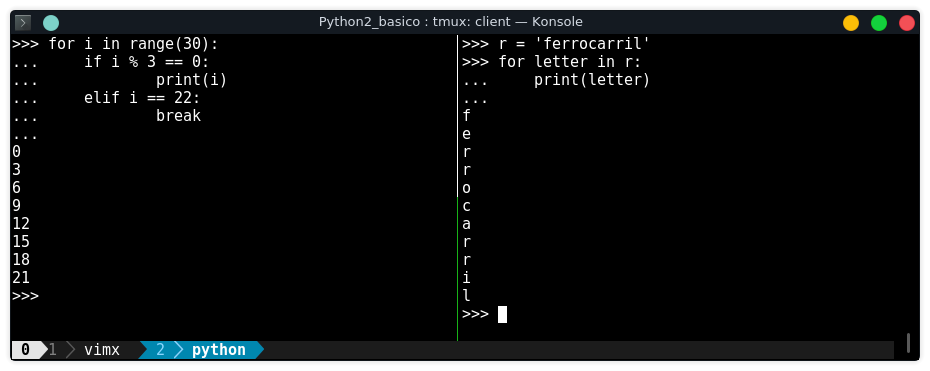
\includegraphics[scale=0.75]{./Pictures/022_for_string.png}
\end{figure}


%% Clase 17
\section{Ciclos en Python con while}%
Otra forma de hacer iteraciones es con el \textbf{while loop}, éste ciclo se
ejecuta MIENTRAS la condición se evalúe como \textbf{verdadera}, el ciclo
termina cuando la evaluación resulta en falso.\\

En este tipo de ciclo es muy importante definir la condición parada, si no el
ciclo puede ejecutarse hasta el infinito y consumir todos los recursos de la
máquina.\\

\begin{figure}[h!]
  \centering
  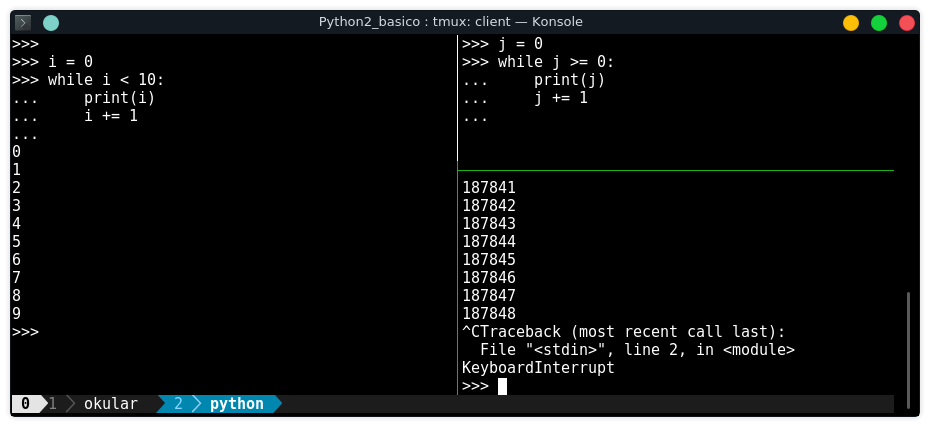
\includegraphics[scale=0.75]{./Pictures/030_while_loop.png}
\end{figure}

\textbf{Recuerda}:
\begin{itemize}
  \item Para detener la ejecución de un ciclo, puede utilizar CTRL + C en la
    consola.
\end{itemize}

Vamos a escribir un programa para adivinar números:\\

\textbf{adivinar\_numero.py}
\begin{minted}{python}
  # -*- coding: utf-8 -*-
  import random


  def run():
      number_found = False
      random_number = random.randint(0, 20)

      while not number_found:
          number = int(raw_input('Intenta un número: '))

          if number == random_number:
              print('Felicidades. Encontraste el número.')
              number_found = True
          elif number > random_number:
              print('El número es más pequeño')
          else:
              print('El número es más grande')


  if __name__ == '__main__':
      run()
\end{minted}

\begin{figure}[h!]
  \centering
  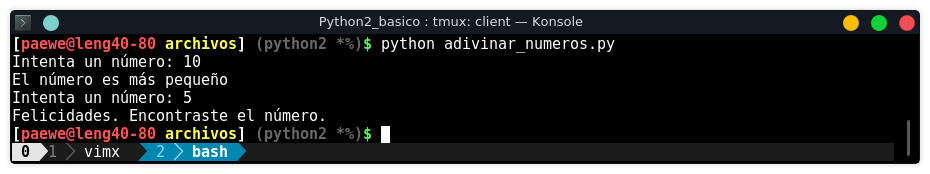
\includegraphics[scale=0.75]{./Pictures/031_adivinar_numero.png}
\end{figure}



%% Clase 18
\section{Calcular si una palabra es palíndromo con Python}%
Creemos un programa para saber si una palabra es un palíndromo. Podemos hacerlo
de muchas formas.\\

\textbf{palindrome.py}
\begin{minted}{python}
  # -*- coding: utf-8 -*-

  def palindrome(word):
      reversed_letters = []

      for letter in word:
          reversed_letters.insert(0, letter)

      reversed_word = ''.join(reversed_letters)

      if reversed_word == word:
          return True

      return False


  if __name__ == '__main__':
      word = str(raw_input('Escribe una palabra: '))

      result = palindrome(word)

      if result is True:
          print('{} sí es un palíndromo.'.format(word))
      else:
          print('{} no es un palíndromo.'.format(word))
\end{minted}

\begin{figure}[h!]
  \centering
  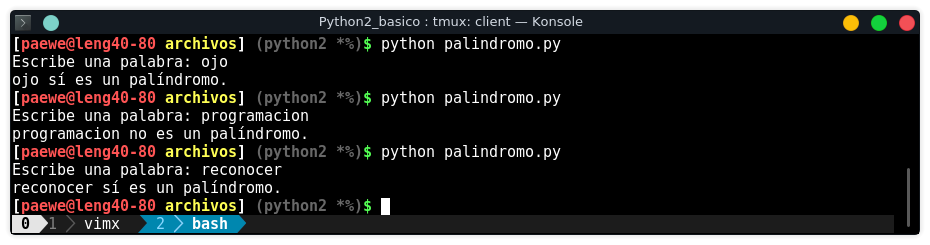
\includegraphics[scale=0.75]{./Pictures/031_palindromo.png}
\end{figure}

\textbf{palindromo2.py}
\begin{minted}{python}
  # -*- coding: utf-8 -*-

  def palindrome(word):
      reversed_word = word[::-1]

      if word == reversed_word:
          return True

      return False


  if __name__ == '__main__':
      word = str(raw_input('Escribe una palabra: '))

      result = palindrome(word)

      if result is True:
          print('{} sí es un palíndromo.'.format(word))
      else:
          print('{} no es un palíndromo.'.format(word))
\end{minted}

\begin{figure}[h!]
  \centering
  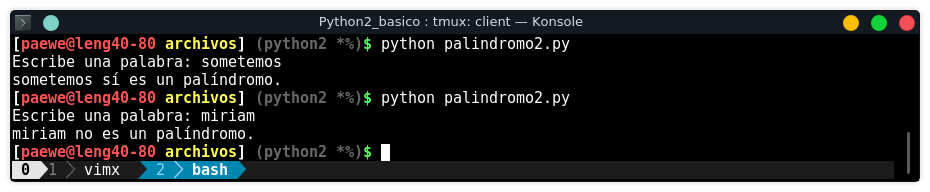
\includegraphics[scale=0.75]{./Pictures/032_palindromo.png}
\end{figure}




%% Clase 19
\section{Introducción a las listas en Python}%
Ya vimos que los strings son una secuencia de caracteres, cuando hablamos de
listas podemos hablar de secuencias de cualquier cosa, por ejemplo listas de
números, listas de strings, listas de objetos más complejos con tipos propios,
etc.\\

Una lista es una secuencia de elementos, para crearlas usamos corchetes $[$ $]$
o con la función \textbf{list}, por ejemplo:\\

Las listas se pueden acceder a través de índices, estos índices inician en cero
(0):

\begin{minted}{python}
  amigos = list()
  numeros = [1, 2, 3, 4, 5]
\end{minted}

Las listas son \textbf{mutables}, para añadir elementos a una lista podemos
utilizar el método \textbf{append}. Las listas se pueden acceder con índices,
que inician en cero.

\begin{minted}{python}
  amigos = list()
  amigos.append('Pedro')
  amigos[0]
  'Pedro'

  amigos.append('Enrique')
  amigos[1]
  'Enrique'
\end{minted}

\begin{figure}[h!]
  \centering
  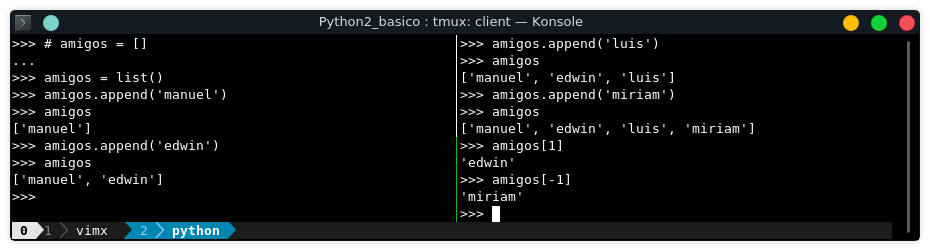
\includegraphics[scale=0.75]{./Pictures/033_listas.png}
\end{figure}

\textbf{average\_temps.py}
\begin{minted}{python}
  # -*- codign: utf-8 -*-


  def average_temps(temps):
      sum_of_temps = 0

      for temp in temps:
          sum_of_temps += float(temp)

      return sum_of_temps / len(temps)


  if __name__ == '__main__':
      temps = [21, 24, 24, 22, 20, 23, 24]

      average = average_temps(temps)

      print('La temperatura promedio es: {}'.format(average))
\end{minted}

\begin{figure}[h!]
  \centering
  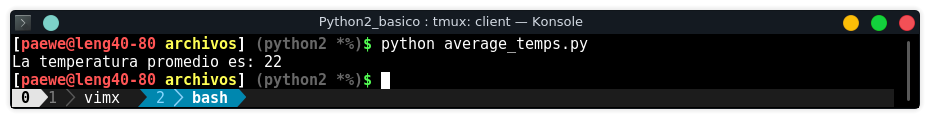
\includegraphics[scale=0.75]{./Pictures/034_average_temp.png}
\end{figure}


%% Clase 20
\section{Operaciones con listas en Python}%
Cuando trabajamos con listas podemos también hacer operaciones por ejemplo:\\

\textbf{Unir listas}
\begin{minted}{python}
  my_list = [1]
  my_list2 = [2, 3, 4]
  my_list3 = my_list + my_list2
  my_list3 # [1, 2, 3, 4]
\end{minted}


\textbf{Multiplicar elementos}
\begin{minted}{python}
  my_lista = ['a']
  my_lista2 = my_lista * 5
  my_lista2 # ['a', 'a', 'a', 'a', 'a']
\end{minted}

\textbf{Dividir listas}
\begin{minted}{python}
  my_lista = [1, 2, 3, 4, 5]
  my_lista_reversed = my_lista[::-1]
  my_lista_reversed # [5, 4, 3, 2, 1]
\end{minted}

\textbf{Eliminar último elemento de la lista}
\begin{minted}{python}
  my_lista = [1, 2, 3, 4, 5]
  my_lista = my_lista.pop()
  my_lista # [1, 2, 3, 4]
\end{minted}

\textbf{Ordenar la lista}
\begin{minted}{python}
  my_lista = [2, 1, 5, 4, 3]
  my_lista = my_lista.sort()
  my_lista # [1, 2, 3, 4, 5]
\end{minted}

\textbf{Eliminar un elemento}
\begin{minted}{python}
  my_lista = [1, 2, 3, 4, 5]
  del my_lista[0]
  my_lista # [2, 3, 4, 5]
\end{minted}






























\end{document}

